%#!platex -kanji=utf8 hb.tex
\chapter{ヒントと今後の動向}\applab{ヒントと今後の動向}
% これはただのダミーテキスト.
% 文字コードを判定するための意味のない文字列.
% これくらい記述すれば大丈夫かな.
% 付録のくせに生意気な.
% 付録の分際で.

\section{プログラム}
\TeX は Donald Knuth氏が1970年代後半から1990年代に開発したプログラムであ
り,そのオリジナルの\TeX から派生したプログラムがいくつも存在します.
\begin{figure}[htbp]
 \begin{center}
  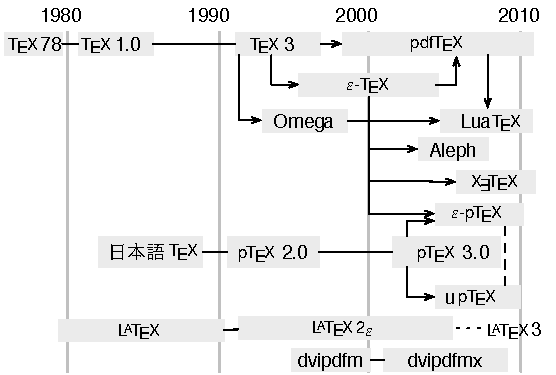
\includegraphics{texhist}
  \caption{簡易的な年表と近年の動向}\figlab{近年の動向}
 \end{center}
\end{figure}
日本語(または中国語,韓国語など)の文字集合を扱うには,\pTeX
のように,独自の拡張を施したプログラムが必要になります.\TeX は世紀を超
えて活用され続けているプログラムであり,また常に改良を加えられているプロ
グラムでもあります.

\subsection{\eTeX}
\TeX というのは \Person{Donald}{Knuth} という\Z{計算機科学者}が何年も前
に開発したプログラムですので,幾分時代にそぐわない部分があると思います.
そこで \TeX を改良した \Prog[eTeX]{\eTeX} なるものが存在します.

現在,北川弘典氏が\eTeX を日本語化した\epTeX\footnote{\webEpTeX}
を公開しております.

%古い記述
%\TeX のレジスタ数を増やしたり,色々と新しいコマンドを追加していたりと便
%利なのですが,\genzai 日本語化されていません\footnote{いくつかのアプロー
%チで日本語を扱う試みはすでにありますが,実用段階にまで達していないのが現状
%です.}.

\subsection{Omega/Aleph}

\TeX を拡張して\Z{多言語組版}を可能にする試みとしては
\Person{John}{Plaice}と\Person{Yannis}{Haralambous}による\Prog{Omega},
\LaTeX 用では \Prog{Lambda}がありました.この後継としては \eTeX をベース
とした \Prog{Aleph}と,\LaTeX 用の\Prog{Lamed}等があります.

\subsection{\PDFTeX}
% H\`an Th\'{\^e} Th\`anh (ハン・タ・タイン).ベトナムの TeXnician
%\url{http://www.tug.org/tug2003/bulletin/souvenirs/photos/TUG2003-Day4-WednesdayJuly23/TUG2003-Day4-WednesdayJuly23-Images/11.jpg}

\TeX から直接 PDF ファイルを作成するためには
\Person{H\`an Th\'{\^e}}{Th\`anh}らによる \Prog[PDFTeX]{\PDFTeX} や
\Prog[PDFlatex]{\PDFLaTeX} というプログラムを使います.これはフォント
メトリクスと実フォント(または仮想フォント)の両方にアクセスする事で一気
にPDFを作成するものです.%\genzai 日本語化されていません.
日本語化についてはまだ実現していません.

\index{LaTeX 3@\LaTeX\,3}%
さらに \eTeX と \PDFTeX をマージして \Prog[PDFeTeX]{\PDFeTeX} というのも
あります.もちろん \Prog[PDFeLaTeX]{\PDFeLaTeX} もあります.
%近い将来 \LaTeXe の後継バージョンである \LaTeX\,3 も登場するでしょうし,
%\PDFTeX が日本語化される日も近いと思われます.

\subsection{\XeTeX}
\PDFeTeX をベースにした\XeTeX\footnote{\webXeTeX}というプログラムもあり
ます.これは OpenTypeフォントに直接アクセスし利用できるようにしたもので
す.近年はLinuxやWindowsでも\XeTeX を使う事ができるようになっています.

\subsection{lua\TeX}
Lua\TeX は{Taco}{Hoekwater},{Hartmut}{Henkel},{Hans}{Hagen}によって
開発されている\PDFTeX の拡張版です.OpenTypeフォントを直接扱う事,また
\MP 画像を直接扱う事ができます.

%\subsection{up\TeX}
%ASCIIによって日本語化された縦組対応の\pTeX の内部コードをUnicode化する
%試みがあります.

%TODO: いるかなぁ
%\subsection{ps2pdf→dvipdfm→dvipdfmx}
%dvipdf   (ps2pdf)
%dvipdfm  1998--2000
%dvipdfmx 2001--2008
%\zindind{デバイス}{ドライバ}%
%近年まで画像は EPS 形式しか受け付けないようなデバイスドライバがあり
%近年は PDF (\W{EPDF}) を直接扱う事ができるdvipdfm,その後継
%のdvipdfmxもありますので,状況はかなり変わっています.状況を考えますと,
%日本語環境では\Dvipdfmx を使うのが最良だと思われます.
%BMP, PNG, JPEG, PDF, EPS 形式の画像の張り込みに対応しています.

\section{フォント}

\subsection{日本語TrueTypeフォント--IPAフォント}
IPAフォント\footnote{\webGRASSIPA}はIPA(独立行政法人情報処理推進機構)
により公開されたJIS~X~0213:2004対応の日本語TrueTypeフォントです.
以下の5書体が用意されています(括弧内はフォント名になります).
\begin{itemize}
 \item IPA~明朝 (ipam.ttf)
 \item IPA~P明朝 (ipamp.ttf)
 \item IPA~ゴシック (ipag.ttf)
 \item IPA~Pゴシック (ipagp.ttf)
 \item IPA~UIゴシック (ipagui.ttf)
\end{itemize}
% Vine マンセー
Vine~Linuxであれば管理者権限にて\type{apt-get install TrueType-ipafont}
とするだけで導入可能です.

%\subsection{TXFonts/PXFonts}
%TODO: すでに他の箇所で説明しているので省略


\subsection{cm-super}
\Person{Donald}{Knuth}がデザインしたComputer ModernフォントはOT1と呼ばれ
るエンーディングの文字集合までしか含まれていません.アクセント類も定義さ
れたT1エンコーディングのフォントをアウトラインフォントでPDFやPostScript
ファイルに埋め込みたいと思った場合,Latin ModernフォントかECフォントの
Type~1形式の{cm-super}フォントを使う事になります.サイズが大きいため,
標準ではインストールされない場合が多いと思われます.
% Vine マンセー
Vine~Linuxであれば管理者権限にて\type{apt-get install ec-fonts-mftraced}
とするだけで導入可能です.

\subsection{OTF}
\index{JIS X 0208@JIS~X~0208}%
\pTeX/\pLaTeX は標準的には JIS X 0208(\Z{JIS 基本漢字})までの\Z{文字
集合}しか扱う事ができません.この問題に関しては\Hito{齋藤}{修三郎}による
\Y{UTF}パッケージで対処できます.\Y{UTF}では \Z{ユニコード} 文字集合まで
扱う事ができます.さらに\Z{Adobe-Japan1-6}までの文字集合に対応した
\Y{OTF}パッケージも開発されています.
% Vine マンセー
Vine~Linuxであれば管理者権限で\type{apt-get install texmacro-otf}
とするだけで導入可能です.

\section{ディストリビューション}
自身のシステムで\LaTeX を使えるようにするには,非常に多くのファイルをイ
ンストールする必要があります.これらを一つに集約したものがディストリビュー
ションと呼ばれるものです.

\subsection{te\TeX}
\Person{Thomas}{Esser}によるte\TeX は,これまで多くのUnix系OSで採用され
てきた\TeX ディストリビューションでした.これをベースに日本語環境を整備
したptetex3\footnote{\webPtetex}が土村展之氏により配布されています.
しかし,te\TeX は2006年に今後の更新は行われないと表明され,現在CTANにお
いてもobsolete扱いになっています.ただし,日本語環境の整備を念頭においた
場合,Unix系OSでは土村氏によるptetex3を選択するのが良いでしょう.

\subsection{\TeX~Live}
\TeX~Liveは\TeX\ Users Groupにより現在でも更新されているディストリビュー
ションです.te\TeX と比較すると非常に巨大なファイル群です.土村氏が
日本語対応を施しているptexliveが開発版として提供されています.

\subsection{W32\TeX}
W32\TeX は角藤亮氏によってメインテナンスされているWindows用の\TeX
ディストリビューションです.更新頻度が非常に早く,数々の改良が加えられて
いるプログラム・ファイルが含まれています.

\section{クラスファイル}

最近までは \W{アスキー} が日本語化した \pTeX に同封されている
\Y{jarticle}, \Y{jreport}, \Y{jbook} を使っていたのですが,現在は\Hito{奥
村}{晴彦}が管理されている \Y{jsclasses} を使うのが良いでしょう.これには
\Y{jsarticle}, \Y{jsbook}, \Y{okumacro}, \Y{okuverb}, \Y{morisawa} など
のクラスとマクロが同封されています.レポートや論文を作成する上でもこれら
のクラス・マクロは非常に完成度が高いため,標準的に\Y{jsclasses}を使う事
を推奨します.
\begin{description}
 \item[\sty{jsarticle}] 
  \sty{jarticle} の代用となるものです.\Option{english} オプションを付け
  る事で,欧文組の時の行送りになります.
 \item[\sty{jsbook}]
  \str{jbook} の代わりとなるもので書籍や論文作成用のクラスとして用います.
  \Option{report} オプションで\sty{jreport}の代用になります.
 \item[okuverb]
  \E{verbatim} 環境をちょっと華麗にするためのパッケージです.
 \item[okumacro]
  奥村氏が美文書作成入門等の著書を執筆するために必要になったマクロを集め
  たものです.
 \item[morisawa]
  モリサワ基本 5 書体パッケージを使うためのマクロです.
\end{description}
ただし,クラスファイルというものは多少なりと製作者の好み等により体裁が調
整されている場合がありますので,自分の求める体裁と差異がある場合は,適宜
該当する箇所を修正する事になります.その方法については本書では言及しませ
ん.

